\section{Delopgave 1}\label{sec:delopgave-1}

\subsection{Relationen \(R\)}\label{subsec:relationen-(r)}

Den følgende graf

\begin{center}
    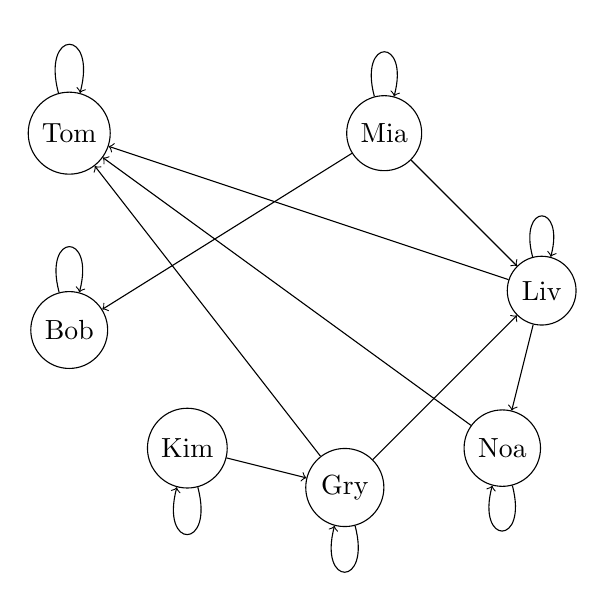
\begin{tikzpicture}
        \node [draw,circle] (Tom) at (0, 0) {Tom};
        \node [draw,circle] (Mia) at (4, 0) {Mia};
        \node [draw,circle] (Liv) at (6, -2) {Liv};
        \node [draw,circle] (Noa) at (5.5, -4) {Noa};
        \node [draw,circle] (Gry) at (3.5, -4.5) {Gry};
        \node [draw,circle] (Kim) at (1.5, -4) {Kim};
        \node [draw,circle] (Bob) at (0, -2.5) {Bob};

        % Reflexive loops
        \draw[->, loop above] (Mia) to (Mia);
        \draw[->, loop above] (Bob) to (Bob);
        \draw[->, loop above] (Liv) to (Liv);
        \draw[->, loop above] (Tom) to (Tom);
        \draw[->, loop below] (Kim) to (Kim);
        \draw[->, loop below] (Gry) to (Gry);
        \draw[->, loop below] (Noa) to (Noa);

        % Edges
        \draw[->] (Mia) -- (Bob);
        \draw[->] (Mia) -- (Liv);
        \draw[->] (Kim) -- (Gry);
        \draw[->] (Gry) -- (Tom);
        \draw[->] (Gry) -- (Liv);
        \draw[->] (Noa) -- (Tom);
        \draw[->] (Liv) -- (Tom);
        \draw[->] (Liv) -- (Noa);
    \end{tikzpicture}
\end{center}

kan også beskrives som relationen \(R\):

\begin{equation}
    \begin{split}
        R =\{\,(\text{Mia}, \text{Mia}), &(\text{Mia}, \text{Bob}), (\text{Mia}, \text{Liv}), (\text{Tom},
        \text{Tom}),\\
        (\text{Bob}, \text{Bob}), & (\text{Kim}, \text{Kim}), (\text{Kim}, \text{Gry}), (\text{Gry}, \text{Gry}), \\
        (\text{Gry}, \text{Tom}), &(\text{Gry}, \text{Liv}), (\text{Noa}, \text{Noa}),(\text{Noa}, \text{Tom}), \\
        (\text{Liv}, \text{Liv}), &(\text{Liv}, \text{Tom}), (\text{Liv}, \text{Noa})\,\}
    \end{split}\label{eq:equation}
\end{equation}

\subsection{Kardinaliteten af relationen \(R\)}\label{subsec:kardinaliteten-af-relationen-(r)}

Kardinaliteten af relationen \(R\) er:

\begin{equation}
    |R| = 15\label{eq:equation5}
\end{equation}

\subsection{\(R\) er en delmængde af et kartesisk produkt}\label{subsec:(r)-er-en-delmngde-af-et-kartesisk-produkt}

Lad \(R\) være en relation og \(A = \{\text{Mia}, \text{Liv}, \text{Noa}, \text{Gry}, \text{Kim}, \text{Bob},
\text{Tom}\}\).
Relationen \(R\) består af ordnede par \((a, b)\) hvor \(a \in A\) og \(b \in A\).

\(R\) kan derfor også defineres som en delmængde af et kartesisk produkt:

\begin{equation}
    R \subseteq A \times A\label{eq:equation3}
\end{equation}

Kardinaliteten af det nævnte kartesiske produkt kan beregnes på følgende måde:

\begin{equation}
    | A \times A | = 49\label{eq:equation4}
\end{equation}

\subsection{Relationens egenskaber}\label{subsec:relationens-egenskaber}

Relationen \(R\) har følgende egenskaber:

\begin{itemize}
    \item \textbf{Refleksiv}: Fordi \(\,\{(a, a) \in R \mid \forall a \in A\,\}\) gælder, dvs.
    for alle elementer i \(A\) er der et tilsvarende element \((a, a)\) i \(R\).
    \item \textbf{Antisymmetrisk}: Fordi \(\forall a, b \in A \) og hvis
    \((a, b) \in R \land (b, a) \in R \implies a = b\).
    I andre ord: Hvis der er et par som fx \((\text{Gry}, \text{Tom})\) i \(R\), må der ikke være et tilsvarende par
    \((\text{Tom}, \text{Gry})\) i \(R\).
    Den eneste undtagelse er hvis \(a = b\).
\end{itemize}

men mangler disse egenskaber:

\begin{itemize}
    \item \textbf{Symmetrisk}: Per definitionen \((a, b) \in R \iff (b, a) \in R \quad\forall a, b \in A\) burde der
    for hvert unikt par \(a, b\) være et tilsvarende par \((b, a)\), fx er der \((\text{Liv}, \text{Tom})\) i \(R\),
    men ikke \((\text{Tom}, \text{Liv})\).
    \item \textbf{Transitiv}: Man kan se at \(R\) ikke er transitiv, bare ved at se at fx
    \((\text{Kim}, \text{Gry})\) og \((\text{Gry}, \text{Liv})\) findes i \(R\), men ikke \((\text{Kim},
    \text{Liv})\).
\end{itemize}

\subsubsection{Hvilken betydning har de forskellige egenskaber for et socialt medie?}

\begin{itemize}
    \item \textbf{Refleksiv}: Man skal følge sig selv.
    \item \textbf{Antisymmetrisk}: Forbindelser er udelukkende ensrettet.
    Dvs.\ man kan ikke følge dem som følger en og omvendt.
    \item \textbf{Symmetrisk}: Man skal være venner, ligesom på Facebook, hvor en forbindelse er gensidig.
    \item \textbf{Transitiv}: Ved at følge en person \(A\), følger man også automatisk alle personer, som \(A\) også
    følger.
\end{itemize}
